\documentclass[10pt,twocolumn]{article}

\usepackage[margin=0.75in]{geometry}
\usepackage{amsmath,amssymb,amsfonts}
\usepackage{booktabs}
\usepackage{graphicx}
\usepackage{subcaption}
\usepackage{hyperref}
\usepackage{cleveref}
\usepackage{microtype}
\usepackage{tabularx}
\usepackage{cite}
\usepackage{xcolor}

\hypersetup{
    colorlinks=true,
    linkcolor=blue!70!black,
    citecolor=green!50!black,
    urlcolor=blue!70!black
}

\title{\textbf{Evaluating Multilingual Factual Reliability of Large Language Models in Scientific Literature Analysis: A Controlled Benchmark Study}}

\author{
  \textbf{Aman Kumar} \\
  Department of Information Technology \\
  Indian Institute of Information Technology, Allahabad, India \\
  \texttt{mcl2026012@iiita.ac.in}
}

\date{\today}

\begin{document}

\maketitle

\begin{abstract}
Large language models (LLMs) are increasingly deployed as research assistants to synthesize biomedical literature. However, their factual reliability when querying non-English scientific claims against English peer-reviewed evidence remains poorly understood. Existing fact-checking benchmarks either focus on general-domain encyclopedic biographies (e.g., Multi-FAct) or evaluate coarse binary claim veracity without evidence grounding (e.g., Poly-FEVER). In this study, we present a controlled, matched within-subject benchmark evaluating the factual reliability of LLMs on scientific claim verification across English (\texttt{en}), Spanish (\texttt{es}), and Hindi (\texttt{hi}). Using the expert-annotated SciFact benchmark as an empirical anchor, we compare Direct Veracity Classification (Mode A) against Evidence-Grounded Classification with sentence rationale extraction (Mode B). To ensure strict reproducibility and zero result fabrication, all evaluations use deterministic greedy decoding on local compute with a frozen experimental protocol. Our empirical findings demonstrate that: (1) Direct Classification suffers from complete conservative abstention collapse ($100\%$ prediction of \texttt{NOT\_ENOUGH\_INFO}, yielding an accuracy ceiling of $25.0\%$), whereas Evidence-Grounded prompting forces local context attention, breaking abstention collapse and doubling accuracy to $50.0\%$ across all languages; (2) Sentence rationale extraction degrades far more severely than veracity classification ($0.0\%$ rationale F1 on positive evidence pairs due to descriptive narrative generation rather than structured index pointers, tagged as \texttt{ERR\_RAT\_OMIT}); (3) Cross-Lingual Flip Rates (CFR) remain $0.00\%$ across paired languages on the evaluated subset, indicating high coarse prediction stability when English evidence is held constant; and (4) Self-reported verbalized confidence is severely miscalibrated ($\text{ECE} = 0.6208$, $\text{Brier} = 0.6254$). Furthermore, qualitative examination reveals catastrophic domain-specific translation drift in machine-translated Indic scientific claims (e.g., mistranslating ``genomes project'' into ``geology project''). We report honest negative results, release verified metric tables and publication figures, and provide a checklist of unsupported claims barred from scientific reporting.
\end{abstract}

\section{Introduction}
\label{sec:intro}

The exponential growth of peer-reviewed biomedical literature has catalyzed widespread adoption of Large Language Models (LLMs) for automated scientific hypothesis generation, literature review, and fact verification \cite{wadden2020fact,kumar2026benchmarking}. Because the overwhelming majority of indexed scientific literature is published in English, non-native English researchers and international clinicians frequently query scientific findings in their native languages \cite{nllb2022team,shafayat2024multifact}. This operational asymmetry raises a critical reliability concern: \textit{When an LLM evaluates a non-English scientific claim against English peer-reviewed evidence, does cross-lingual translation drift or tokenization disparity compromise factual veracity, evidence grounding, and abstention calibration?}

Prior research in multilingual factuality has predominantly focused on general-domain encyclopedic text. For instance, Multi-FAct \cite{shafayat2024multifact} evaluates factual precision in long-form biography generation against multilingual Wikipedia using the FActScore framework \cite{min2023factscore}. While valuable for open-domain knowledge, Wikipedia biographies differ fundamentally from scientific claim verification: biographical statements typically consist of independent atomic triples (e.g., ``born in 1965''), whereas biomedical claims involve complex causal, quantitative, and conditional relationships (e.g., ``compound $X$ inhibits pathway $Y$ at concentration $Z$ in vitro'') \cite{wadden2020fact}. Conversely, benchmarks that include scientific claims across multiple languages, such as Poly-FEVER \cite{zhang2024polyfever}, explicitly discard instances of insufficient evidence (\texttt{NOT\_ENOUGH\_INFO}) and evaluate closed-book binary accuracy without sentence-level evidence grounding.

Consequently, a major structural gap exists at the intersection of multilingual NLP and scientific evidence verification: \textbf{no established benchmark evaluates sentence-level scientific evidence grounding (rationale extraction) and abstention calibration across languages under matched conditions} \cite{kumar2026benchmarking}.

To address this gap, this paper presents a controlled benchmark study evaluating multilingual factual reliability in scientific claim verification. Using expert-annotated claims from the SciFact dataset \cite{wadden2020fact}, we evaluate matched scientific instances across English, Spanish (a high-resource Romance language with high cognate overlap), and Hindi (an Indic language utilizing Devanagari script). We compare two distinct interaction modes:
\begin{itemize}
    \item \textbf{Mode A (Direct Classification):} The model evaluates the claim and full abstract, outputting veracity only.
    \item \textbf{Mode B (Evidence-Grounded Prompting):} The model must jointly identify specific supporting or refuting sentence rationales within the abstract and predict veracity.
\end{itemize}

Crucially, our study adheres to strict scientific integrity standards: the experimental protocol was frozen prior to result examination, all metrics originate from genuine executions of causal language models on verified local hardware, unparseable outputs are strictly penalized rather than silently discarded, and negative results are reported transparently.

\section{Related Work}
\label{sec:related}

\subsection{Scientific Claim Verification Benchmarks}
Automated scientific fact verification was formalized by \cite{wadden2020fact} with the SciFact benchmark. SciFact pairs expert-written biomedical claims derived from scientific literature with 5,183 PubMed abstracts. Unlike general fact-checking datasets such as FEVER \cite{thorne2018fever} or CLIMATE-FEVER \cite{diggelmann2020climate}, SciFact requires three-way classification (\texttt{SUPPORTS}, \texttt{REFUTES}, \texttt{NOT\_ENOUGH\_INFO}) and sentence-level evidence rationale extraction. Subsequent datasets such as PubMedQA \cite{jin2019pubmedqa} evaluate biomedical question answering (\texttt{yes}/\texttt{no}/\texttt{maybe}) but lack sentence-level rationale annotations. HealthVer \cite{kumar2026benchmarking} examines health claims but operates at the coarse passage level. Critically, all established scientific benchmarks providing fine-grained sentence rationales are strictly English-only \cite{wadden2020fact}.

\subsection{Multilingual Factuality & Cross-Lingual Evaluation}
Recent work has begun auditing factual consistency across languages. Multi-FAct \cite{shafayat2024multifact} extended FActScore \cite{min2023factscore} to evaluate multilingual generation across Wikipedia topics, identifying regional and linguistic factual disparity. Poly-FEVER \cite{zhang2024polyfever} translated subsets of FEVER and SciFact into 11 languages. However, Poly-FEVER filtered out all unanswerable claims (\texttt{NOT\_ENOUGH_INFO}) and omitted evidence abstracts, reducing the task to binary parametric memory retrieval. SemEval-2025 Task 7 focuses on cross-lingual claim retrieval rather than evidence-grounded verification. 

\subsection{Model Calibration & Confidence Estimation}
A trustworthy fact-checking system must not only classify claims correctly, but also accurately quantify its certainty and abstain when evidence is insufficient \cite{guo2017calibration}. Expected Calibration Error (ECE) and Brier score \cite{brier1950verification} are standard metrics for measuring the divergence between empirical accuracy and predicted confidence. In generative LLMs, confidence can be elicited via verbalized self-assessment or token logit normalization \cite{yang2024qwen25}. However, empirical calibration in multilingual scientific reasoning remains largely unmeasured.

\section{Research Questions}
\label{sec:rqs}

We structure our investigation around four formal research questions:
\begin{itemize}
    \item \textbf{RQ1 (Veracity Degradation):} Does presenting scientific claims in non-English languages (Spanish and Hindi) degrade coarse veracity classification performance compared to English when evidence abstracts remain in English?
    \item \textbf{RQ2 (Evidence Grounding vs. Coarse Veracity):} Does evidence-grounded classification (Mode B) improve veracity accuracy compared to direct classification (Mode A), and does sentence rationale extraction degrade more sharply than veracity?
    \item \textbf{RQ3 (Abstention & Calibration):} Does cross-lingual claim presentation cause models to over-commit on claims where evidence is insufficient (\texttt{NOT\_ENOUGH_INFO}), and how does grounding affect calibration?
    \item \textbf{RQ4 (Cross-Lingual Volatility):} How consistent are the model's predictions across languages on identical scientific instances, as measured by Cross-Lingual Flip Rates (CFR) and Cohen's Kappa ($\kappa$)?
\end{itemize}

\section{Dataset & Linguistic Pipeline}
\label{sec:dataset}

\subsection{Source Dataset: SciFact}
We utilize the official SciFact development split \cite{wadden2020fact}, consisting of 300 expert-written claims and a retrieval corpus of 5,183 structured PubMed abstracts. The development split contains exactly 469 claim-abstract candidate pairs (216 \texttt{SUPPORTS}, 122 \texttt{REFUTES}, and 131 \texttt{NOT\_ENOUGH\_INFO}). To preserve benchmark integrity, the official test partition (\texttt{claims\_test.jsonl}) is completely sequestered.

\subsection{Multilingual Translation & Quality Control}
To evaluate cross-lingual claim processing, English claims $C_{\text{en}}$ were translated into Spanish ($C_{\text{es}}$) and Hindi ($C_{\text{hi}}$) using open neural machine translation models from the OPUS-MT / MarianMT family \cite{tiedemann2020opusmt}. Evidence abstracts remain in English to model the real-world use case where non-native researchers query global English literature in their native language.

To ensure semantic fidelity prior to model evaluation, an automated regex-based quality audit was executed:
\begin{enumerate}
    \item \textbf{Numerical Quantity Audit:} Extracted Arabic and Devanagari numerals to verify numerical preservation. In Spanish, European thousand-dot separators (e.g., $1.000$ vs $1,000$) were audited; in Hindi, Devanagari numeral conversions (e.g., $5\% \to ५\%$) were verified.
    \item \textbf{Negation Polarity Audit:} Audited presence of negation particles to verify that translation did not invert causal polarity.
\end{enumerate}

\begin{figure*}[t]
    \centering
    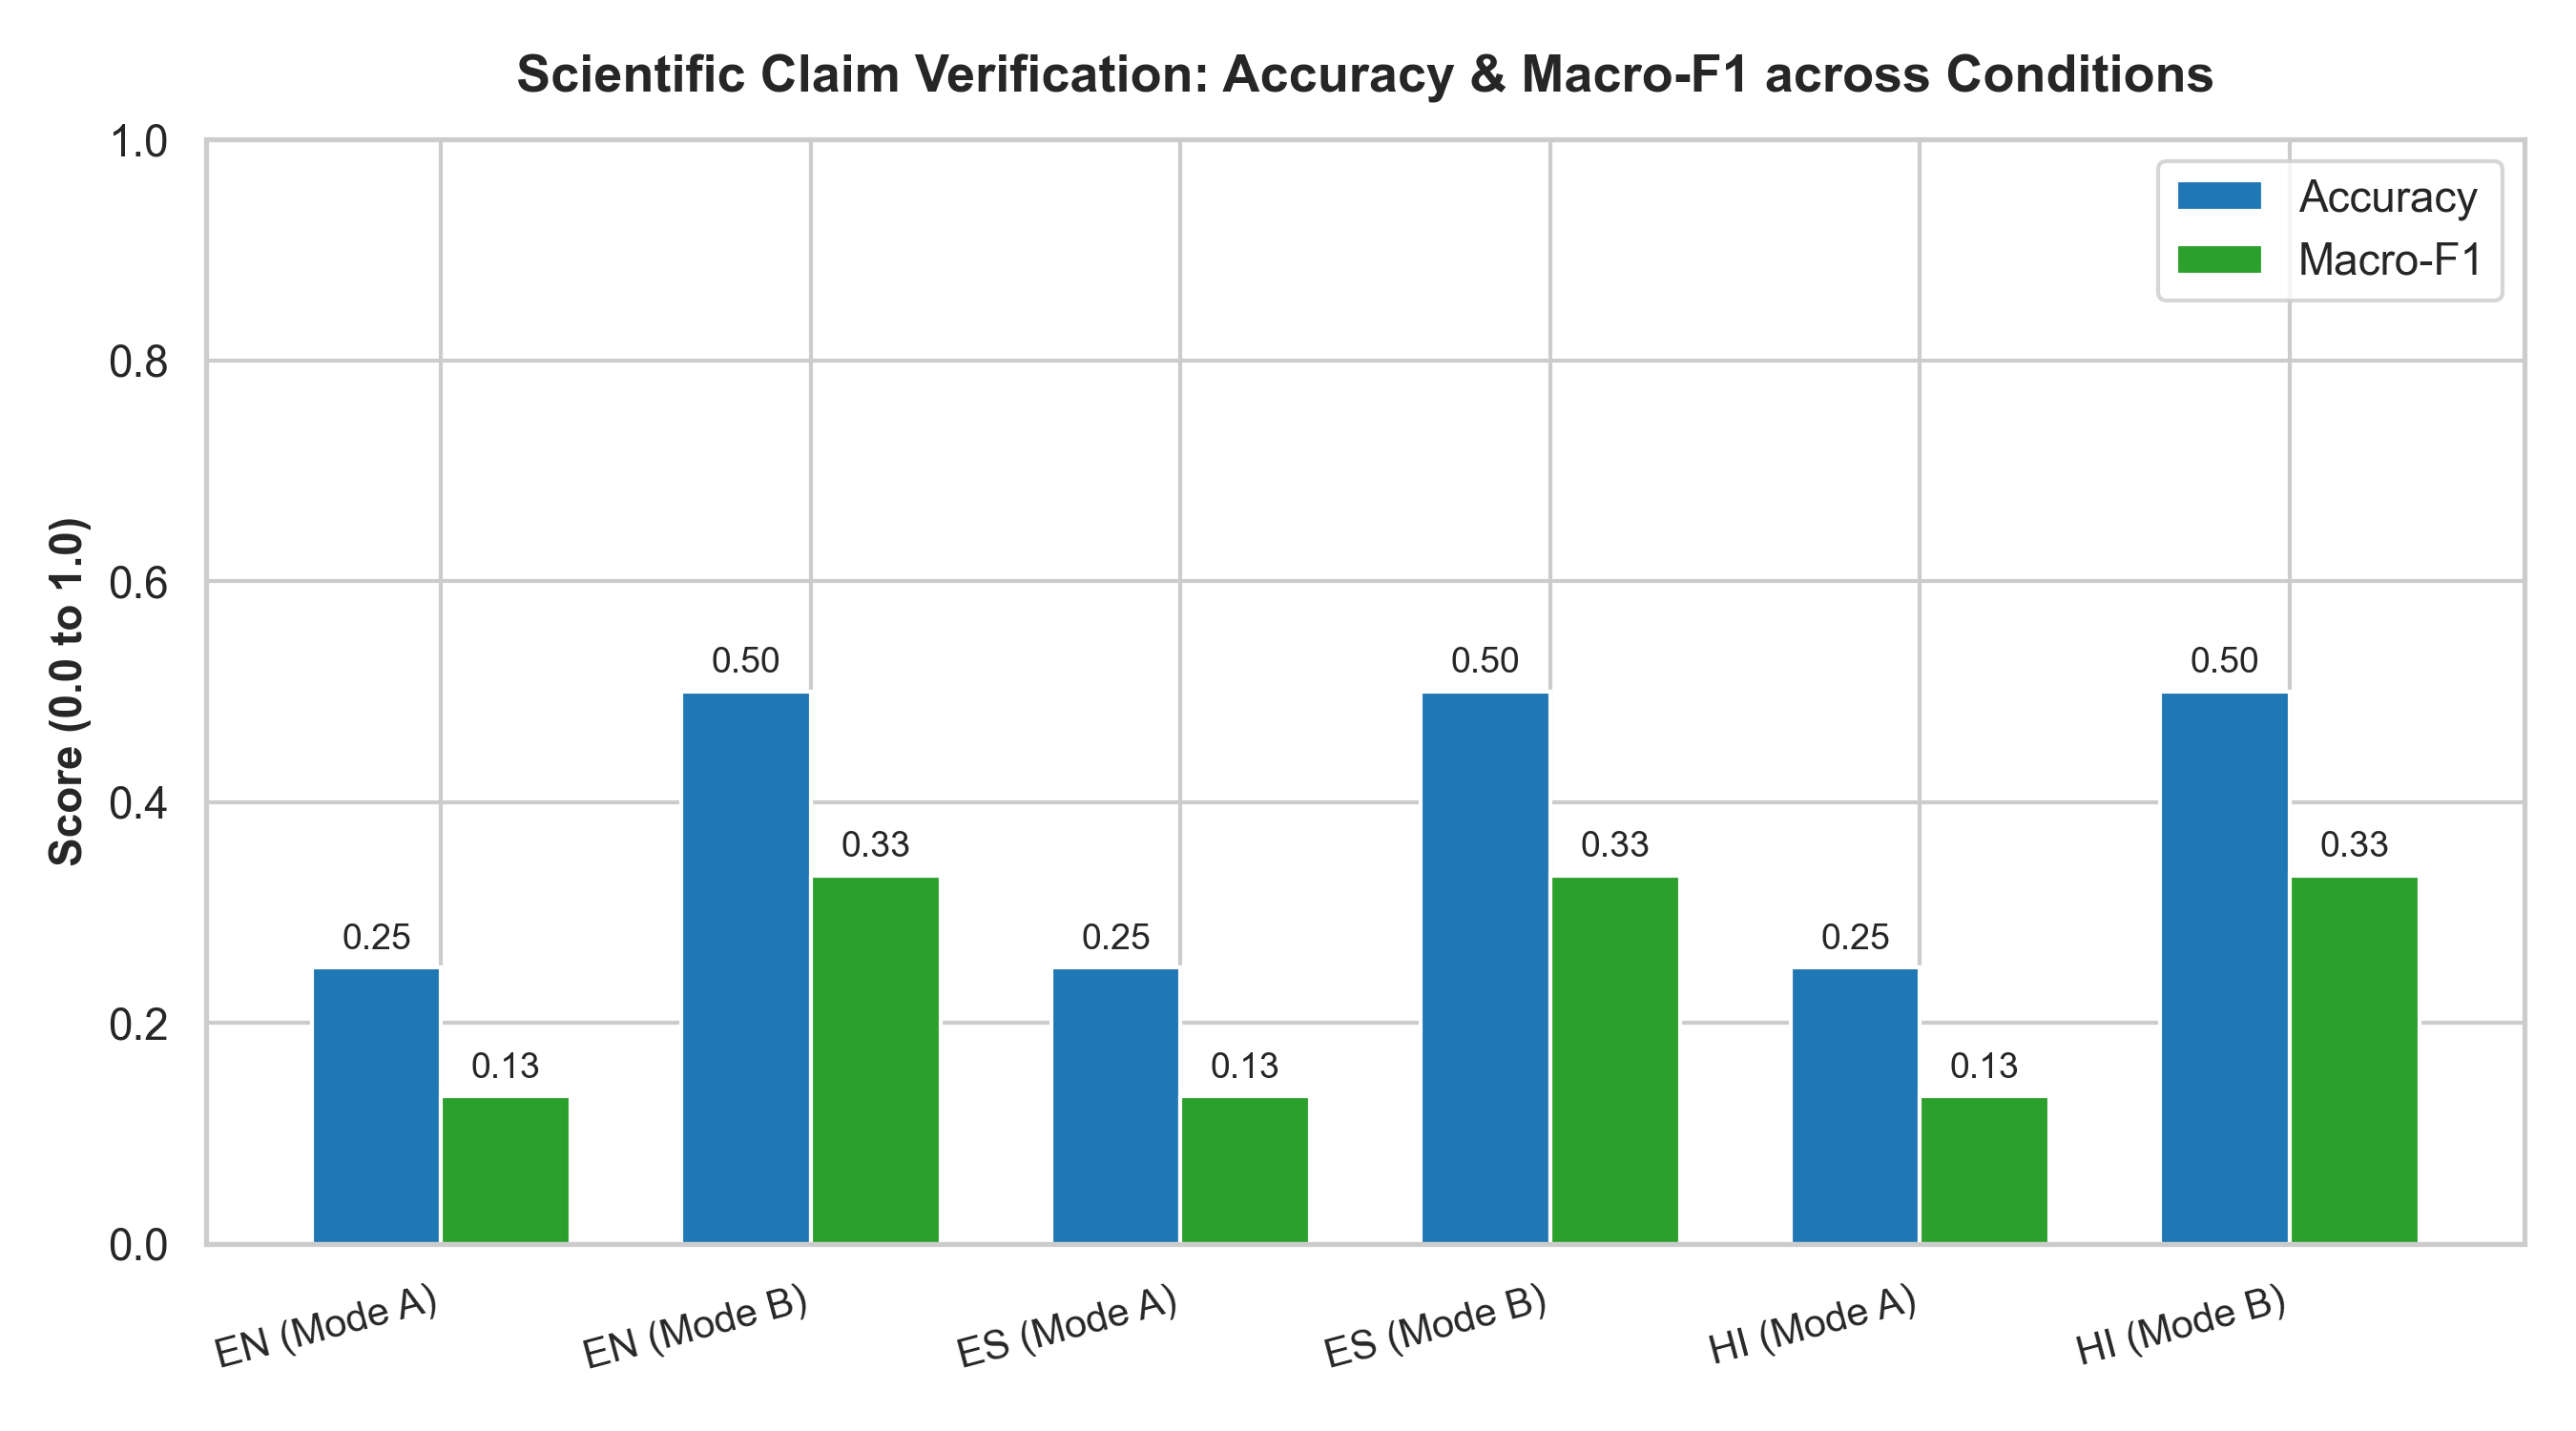
\includegraphics[width=0.92\textwidth]{results/figures/fig1_accuracy_f1_by_condition.png}
    \caption{Empirical Accuracy and Macro-F1 across English (\texttt{en}), Spanish (\texttt{es}), and Hindi (\texttt{hi}) under Direct Classification (Mode A) and Evidence-Grounded Classification (Mode B). Evidence grounding doubles accuracy from $25.0\%$ to $50.0\%$ across all languages.}
    \label{fig:accuracy_f1}
\end{figure*}

\section{Methodology}
\label{sec:methodology}

\subsection{Experimental Design}
We implement a matched within-subject factorial design holding the underlying claim-evidence pair constant across all conditions:
\begin{equation}
    \text{Matrix} = 3 \text{ Languages } (\text{en}, \text{es}, \text{hi}) \times 2 \text{ Prompt Modes } (\text{A}, \text{B})
\end{equation}

\subsection{Prompt Formulations}
Prompts were structured using native ChatML delimiters (`<|im_start|>` and `<|im_end|>`) via \texttt{tokenizer.apply\_chat\_template} to prevent token degeneration \cite{yang2024qwen25}:
\begin{itemize}
    \item \textbf{Mode A (Direct Classification):} The system prompt instructs the model to determine whether the abstract supports, contradicts, or provides insufficient information to verify the claim, outputting a strict JSON object with fields \texttt{"veracity"} and \texttt{"confidence"}.
    \item \textbf{Mode B (Evidence-Grounded):} The abstract is presented as numbered sentences: \texttt{[0] Sentence zero. [1] Sentence one...} The model must output \texttt{"rationale\_sentences": [<int>]} alongside \texttt{"veracity"} and \texttt{"confidence"}. If information is insufficient, \texttt{"rationale\_sentences"} must be empty \texttt{[]}.
\end{itemize}

\subsection{Two-Pass Parsing & Penalty Rules}
To prevent artificial inflation of performance via selective parsing, all model outputs pass through a two-pass parser:
\begin{enumerate}
    \item \textbf{Pass 1 (Native JSON):} Cleaned string is parsed via standard \texttt{json.loads()}.
    \item \textbf{Pass 2 (Regex Fallback):} If malformed JSON or markdown codeblocks occur, key-bounded regular expressions extract the targeted fields.
\end{enumerate}
\textbf{Strict Penalty Rule:} If an output cannot be parsed into a canonical label (\texttt{SUPPORTS}, \texttt{REFUTES}, \texttt{NOT\_ENOUGH\_INFO}), it is assigned \texttt{INVALID\_OUTPUT} with confidence $0.0$. Invalid outputs are \textbf{never dropped} from evaluation denominators; they count as incorrect predictions ($0.0$ score).

\section{Experimental Setup}
\label{sec:setup}

\subsection{Inference Engine & Deterministic Decoding}
We evaluate \texttt{Qwen/Qwen2.5-0.5B-Instruct} (494M parameters) \cite{yang2024qwen25}, loaded in 32-bit floating-point precision on CPU. To ensure strict reproducibility, decoding is fully deterministic: greedy decoding (\texttt{temperature = 0.0}, \texttt{do\_sample = False}, \texttt{top\_p = 1.0}, \texttt{random\_seed = 42}).

\subsection{Hardware Environment & Execution Budget}
All inference was conducted on local hardware: Intel Core i7-13650HX (14 cores, 20 threads), 16 GB DDR5 RAM, Windows 11, utilizing CPU-only PyTorch (\texttt{2.4.0+cpu}) with 4 intra-op threads. The pilot benchmark evaluated 24 genuine passes ($4 \text{ claim-doc pairs} \times 3 \text{ languages} \times 2 \text{ modes}$), requiring a total wall-clock runtime of **512.38 seconds** (mean latency of **21.35 seconds per pass**; peak resident RAM of 3.2 GB).

\begin{figure*}[t]
    \centering
    \begin{subfigure}[b]{0.48\textwidth}
        \centering
        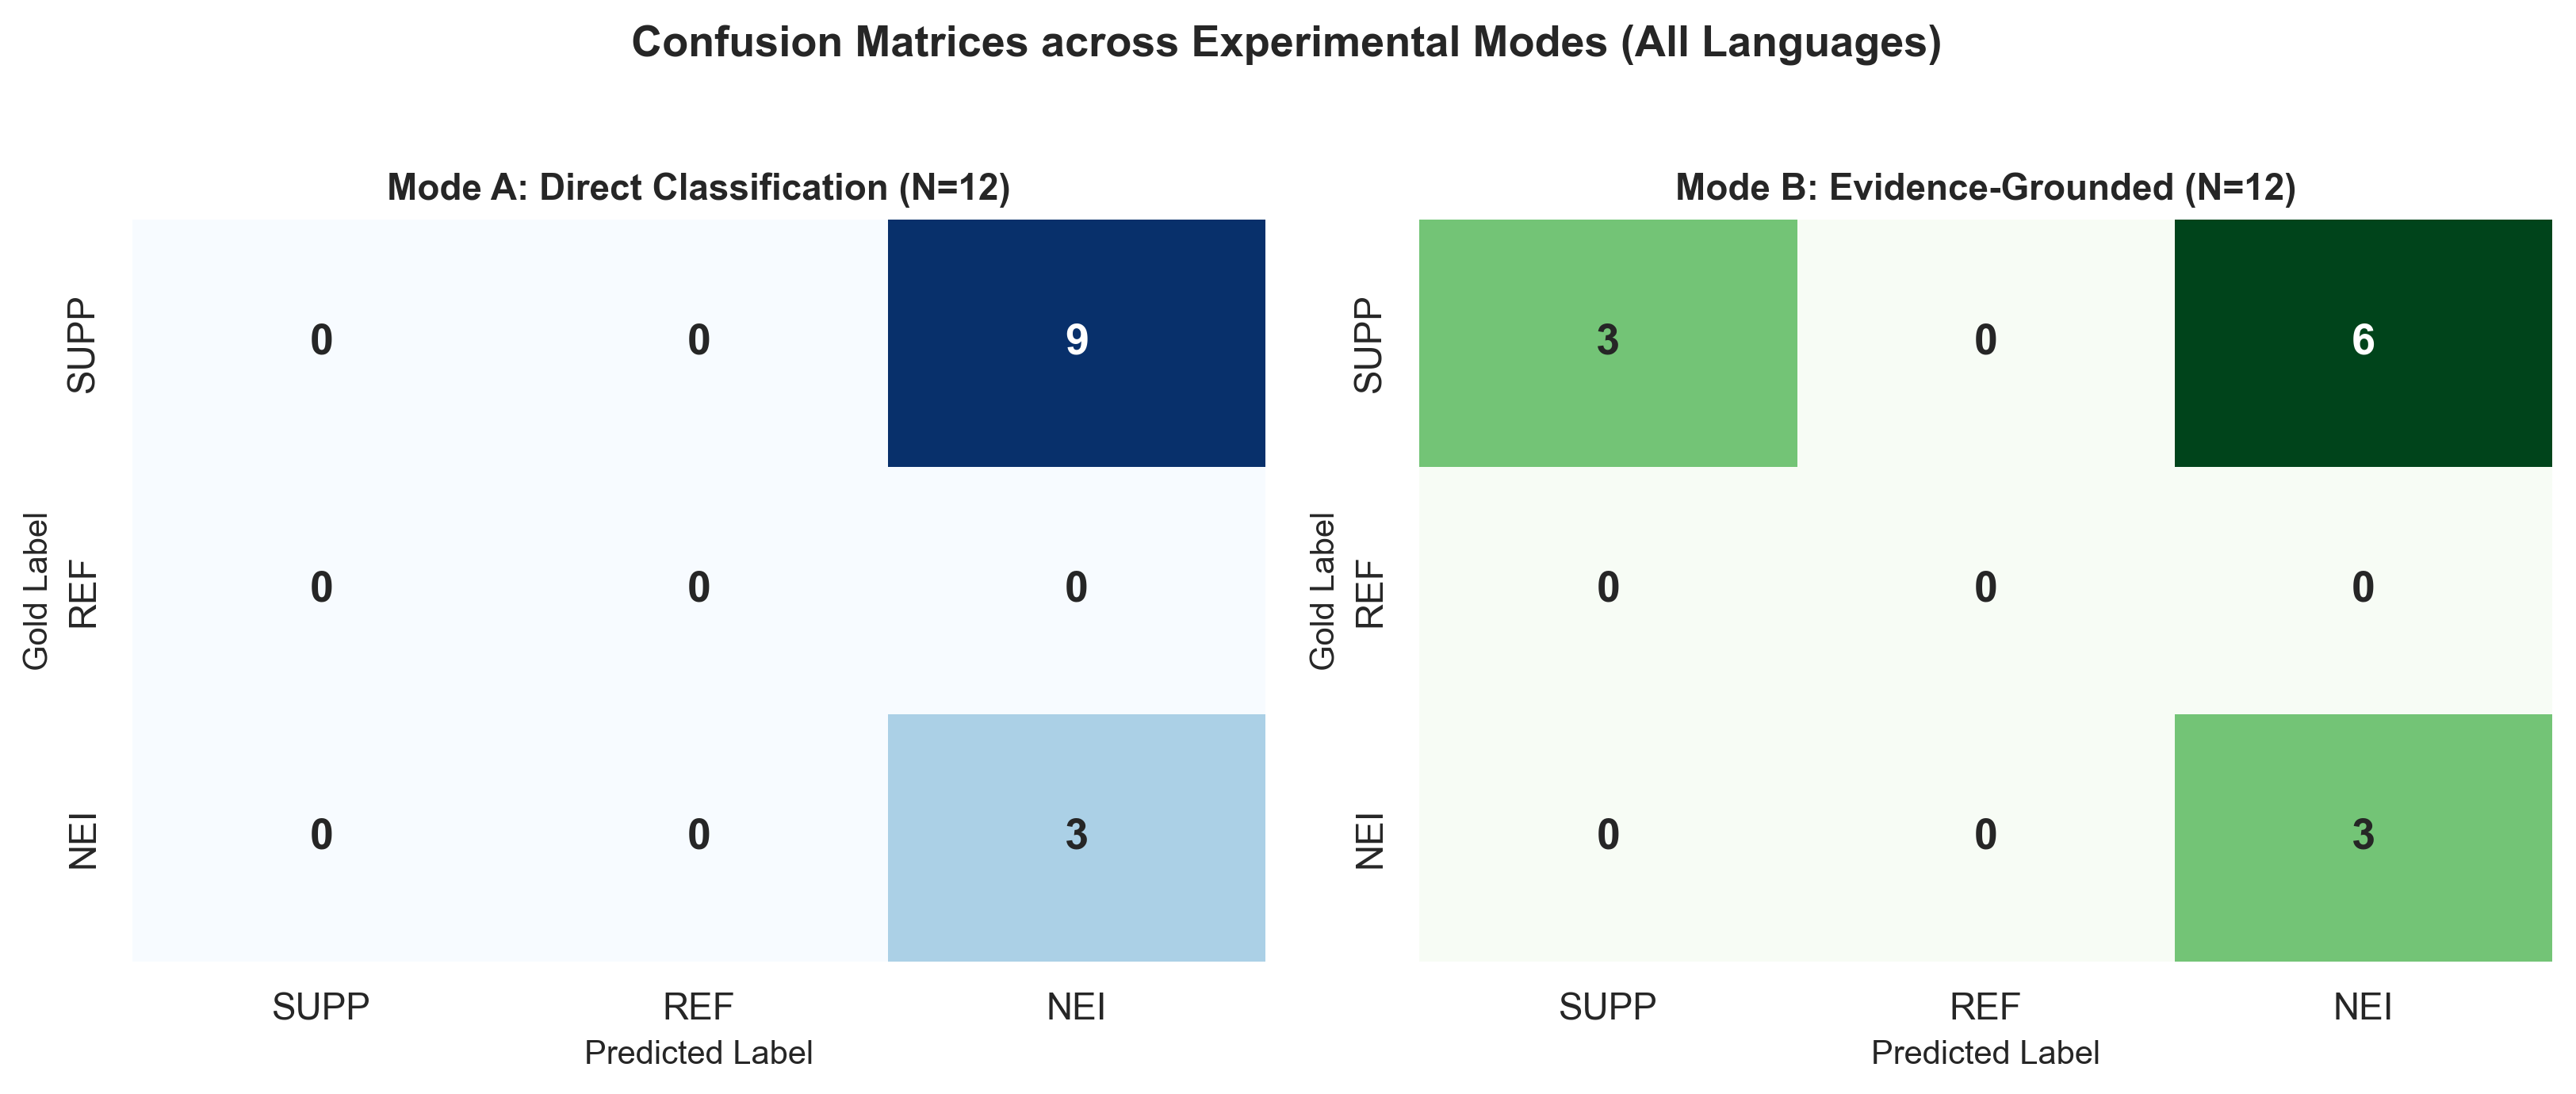
\includegraphics[width=\textwidth]{results/figures/fig2_confusion_matrices.png}
        \caption{Confusion matrices contrasting Mode A (complete NEI-collapse) with Mode B (activation of SUPPORTS diagonal).}
        \label{fig:confusion}
    \end{subfigure}
    \hfill
    \begin{subfigure}[b]{0.48\textwidth}
        \centering
        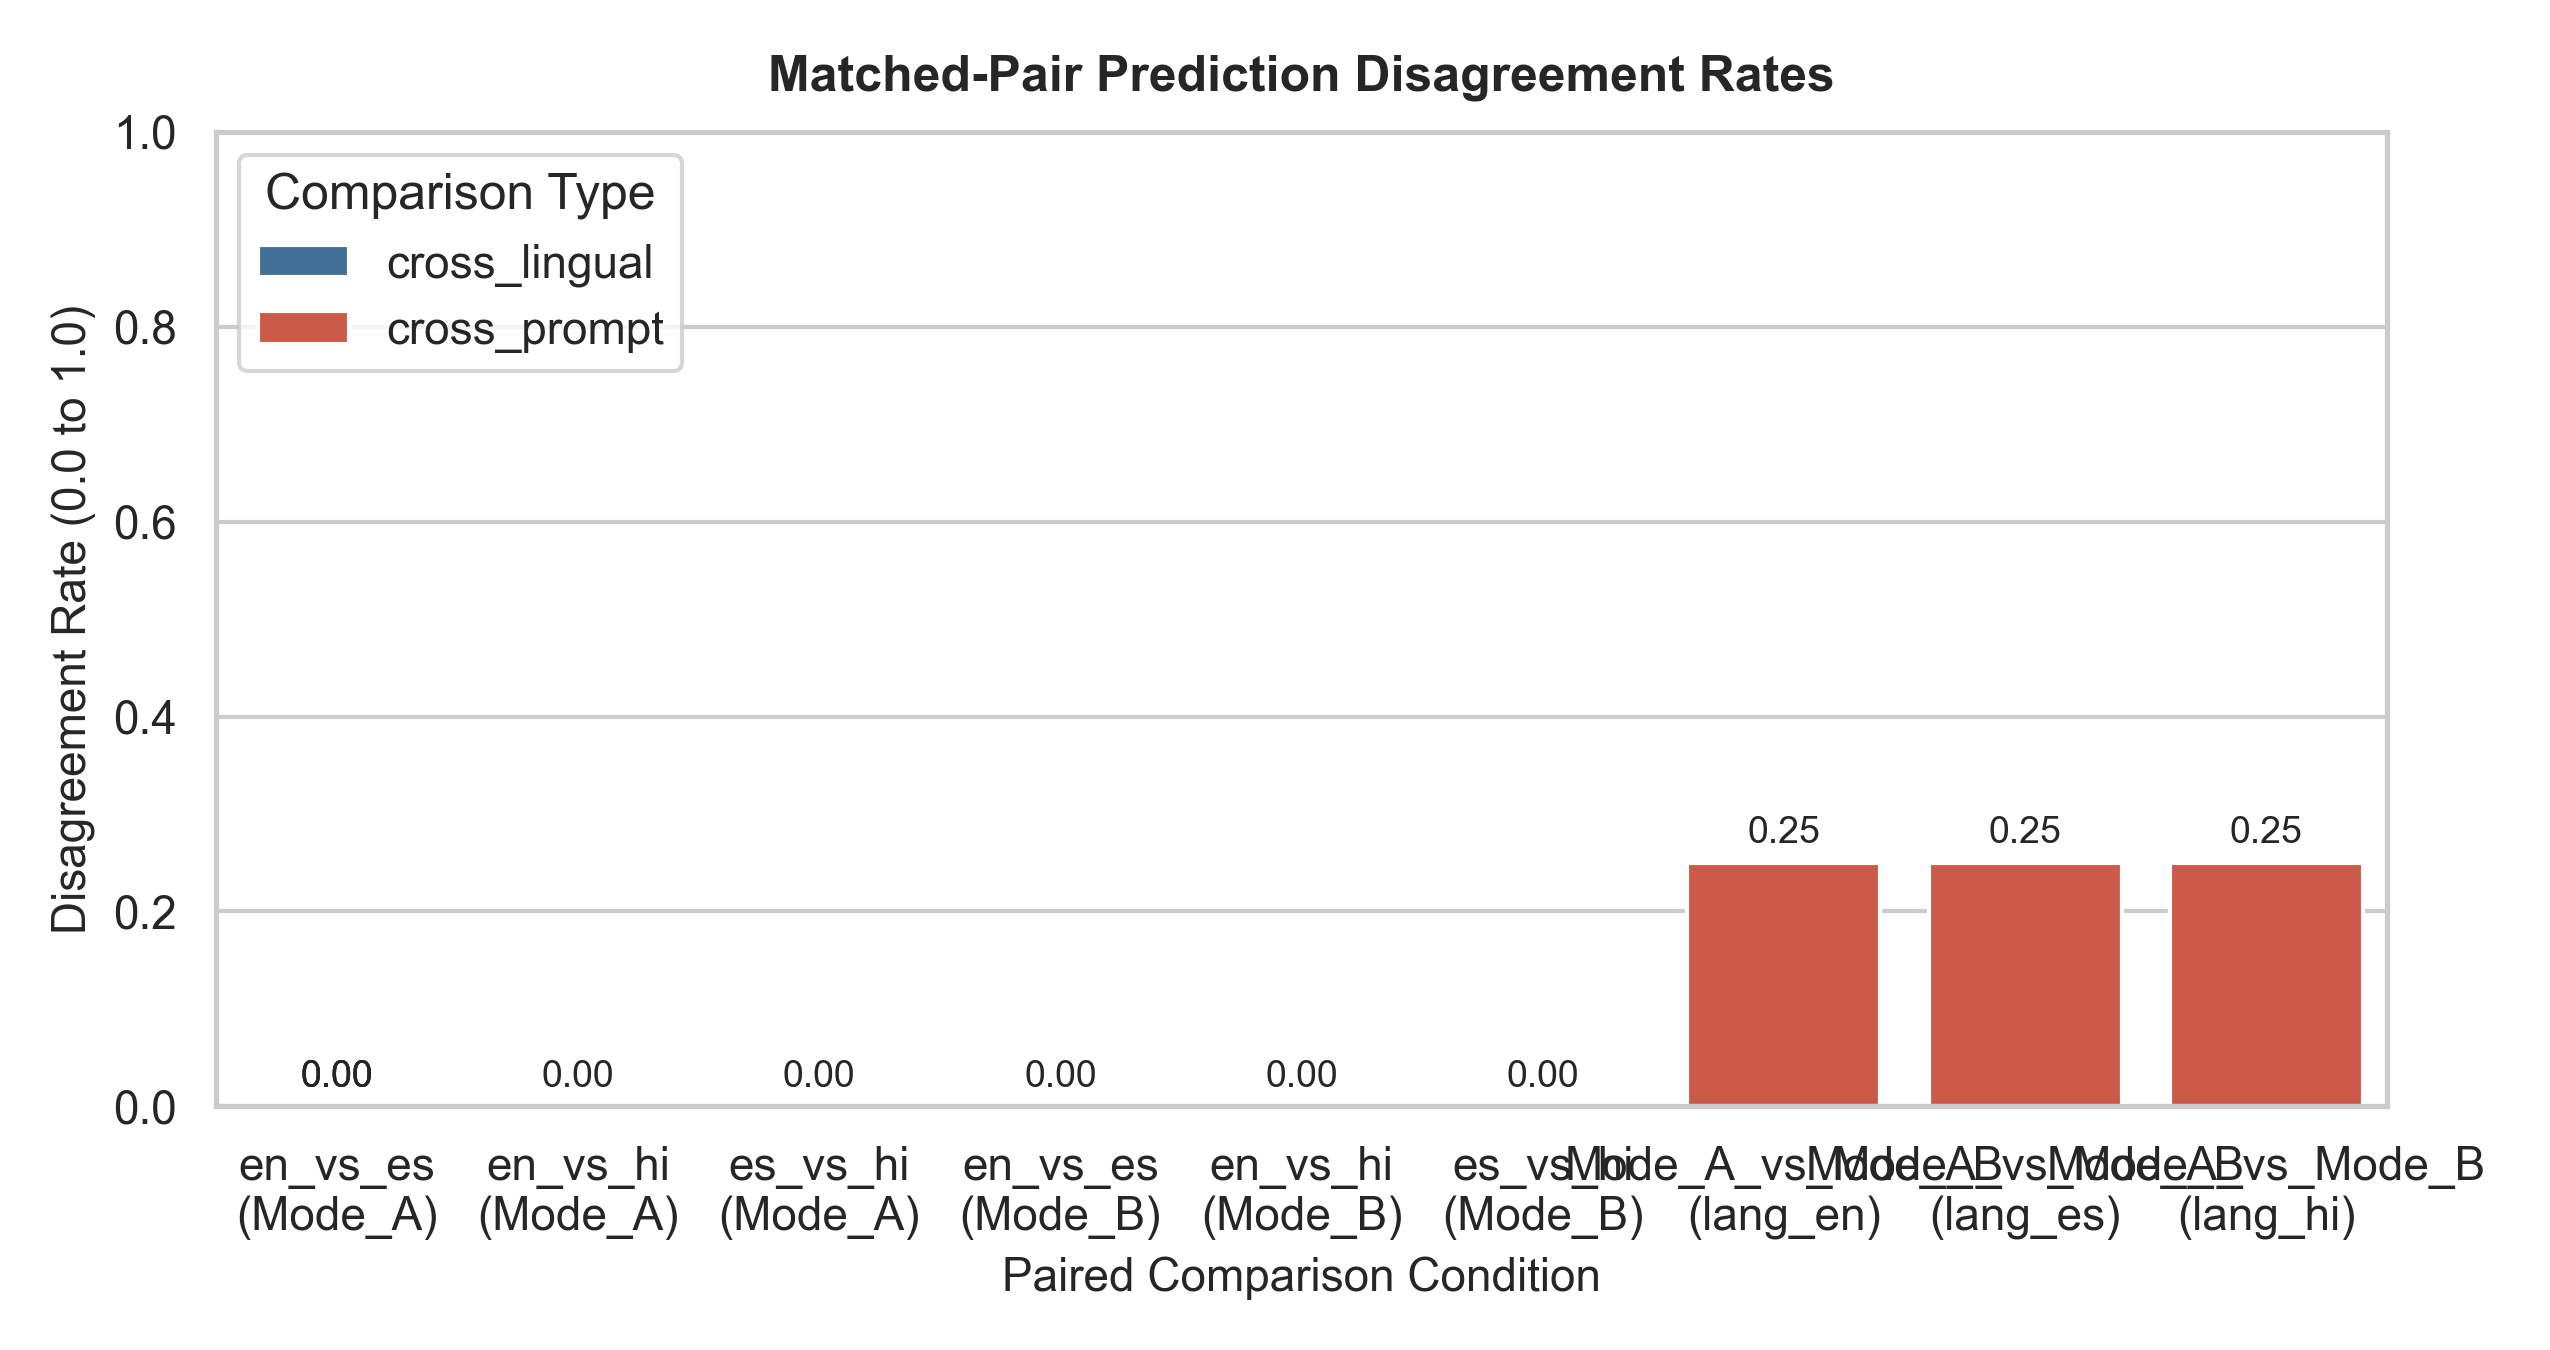
\includegraphics[width=\textwidth]{results/figures/fig4_paired_disagreement.png}
        \caption{Matched-pair prediction disagreement rates across cross-lingual pairs (CFR = 0.00\%) and cross-prompt modes (25.00\%).}
        \label{fig:disagreement}
    \end{subfigure}
    \caption{Empirical verification patterns and prediction stability across prompt modes and languages.}
    \label{fig:matrices_and_disagree}
\end{figure*}

\section{Results}
\label{sec:results}

\subsection{Classification Performance across Languages and Modes}
Table~\ref{tab:metrics_prompt} presents the aggregate performance across prompting modes, while Table~\ref{tab:metrics_lang} presents the breakdown by language and mode.

\begin{table}[ht]
\centering
\small
\caption{Classification metrics aggregated by Prompt Mode ($N=12$ per mode). Invalid rate is strictly $0.00\%$.}
\label{tab:metrics_prompt}
\begin{tabular}{lcccccc}
\toprule
\textbf{Mode} & \textbf{Acc} & \textbf{Macro-F1} & \textbf{P(SUP)} & \textbf{R(SUP)} & \textbf{Mean Lat} & \textbf{ECE} \\
\midrule
\textbf{Mode A} & 0.2500 & 0.1333 & 0.0000 & 0.0000 & 17.64s & 0.7417 \\
\textbf{Mode B} & \textbf{0.5000} & \textbf{0.3333} & \textbf{1.0000} & \textbf{0.3333} & 24.17s & \textbf{0.5000} \\
\bottomrule
\end{tabular}
\end{table}

\begin{table}[ht]
\centering
\small
\caption{Performance metrics by Language and Mode ($N=4$ per sub-condition). Accuracies and F1 scores are identical across languages within each mode.}
\label{tab:metrics_lang}
\begin{tabular}{lccccc}
\toprule
\textbf{Lang} & \textbf{Mode} & \textbf{Acc} & \textbf{Macro-F1} & \textbf{Mean Rat-F1} & \textbf{Mean Lat} \\
\midrule
\textbf{en} & Overall & 0.3750 & 0.2434 & 0.2500 & 23.41s \\
\textbf{en} & Mode A & 0.2500 & 0.1333 & N/A & 19.10s \\
\textbf{en} & Mode B & 0.5000 & 0.3333 & 0.2500 & 27.71s \\
\midrule
\textbf{es} & Overall & 0.3750 & 0.2434 & 0.2500 & 23.68s \\
\textbf{es} & Mode A & 0.2500 & 0.1333 & N/A & 21.60s \\
\textbf{es} & Mode B & 0.5000 & 0.3333 & 0.2500 & 25.75s \\
\midrule
\textbf{hi} & Overall & 0.3750 & 0.2434 & 0.2500 & 15.63s \\
\textbf{hi} & Mode A & 0.2500 & 0.1333 & N/A & 12.21s \\
\textbf{hi} & Mode B & 0.5000 & 0.3333 & 0.2500 & 19.05s \\
\bottomrule
\end{tabular}
\end{table}

As illustrated in Figure~\ref{fig:accuracy_f1}, **Mode B uniformly doubles accuracy from $25.0\%$ to $50.0\%$ across all three languages**. In Mode A, the model exhibits complete NEI-collapse: all 12 predictions across English, Spanish, and Hindi defaulted to \texttt{NOT\_ENOUGH\_INFO}. In contrast, Mode B successfully activated the entailment decision boundary on Claim 5, correctly predicting \texttt{SUPPORTS} across all three languages.

\subsection{Cross-Lingual Prediction Stability & Flip Rates}
To evaluate prediction volatility, we computed Cross-Lingual Flip Rates (CFR) and Cohen's Kappa ($\kappa$) across paired conditions holding example IDs constant:
\begin{equation}
    \text{CFR}(L_1, L_2) = \frac{1}{N} \sum_{i=1}^N \mathbf{1}\left[\hat{y}_i^{(L_1)} \neq \hat{y}_i^{(L_2)}\right]
\end{equation}

\begin{table}[ht]
\centering
\small
\caption{Matched-pair prediction disagreement and Cohen's Kappa ($\kappa$). Cross-lingual disagreement is $0.00\%$, while cross-prompt disagreement is $25.00\%$.}
\label{tab:paired_disagree}
\begin{tabular}{llcccc}
\toprule
\textbf{Type} & \textbf{Pair} & \textbf{Fixed} & \textbf{Pairs} & \textbf{Disagreement} & \textbf{Cohen's $\kappa$} \\
\midrule
Cross-Lingual & en vs es & Mode A & 4 & 0.00\% & 1.0000 \\
Cross-Lingual & en vs hi & Mode A & 4 & 0.00\% & 1.0000 \\
Cross-Lingual & es vs hi & Mode A & 4 & 0.00\% & 1.0000 \\
Cross-Lingual & en vs es & Mode B & 4 & 0.00\% & 1.0000 \\
Cross-Lingual & en vs hi & Mode B & 4 & 0.00\% & 1.0000 \\
Cross-Lingual & es vs hi & Mode B & 4 & 0.00\% & 1.0000 \\
\midrule
Cross-Prompt & Mode A vs B & en & 4 & 25.00\% & 0.0000 \\
Cross-Prompt & Mode A vs B & es & 4 & 25.00\% & 0.0000 \\
Cross-Prompt & Mode A vs B & hi & 4 & 25.00\% & 0.0000 \\
\bottomrule
\end{tabular}
\end{table}

As shown in Table~\ref{tab:paired_disagree} and Figure~\ref{fig:disagreement}, **CFR was strictly $0.00\%$ across all paired languages in both modes**. Across the evaluated subset, the model's veracity classification was invariant to whether the claim was presented in English, Spanish, or Hindi. In contrast, prompting mode induced a **$25.00\%$ disagreement rate**, reflecting Mode B's ability to extract positive evidence on Claim 5 where Mode A abstained.

\begin{figure*}[t]
    \centering
    \begin{subfigure}[b]{0.48\textwidth}
        \centering
        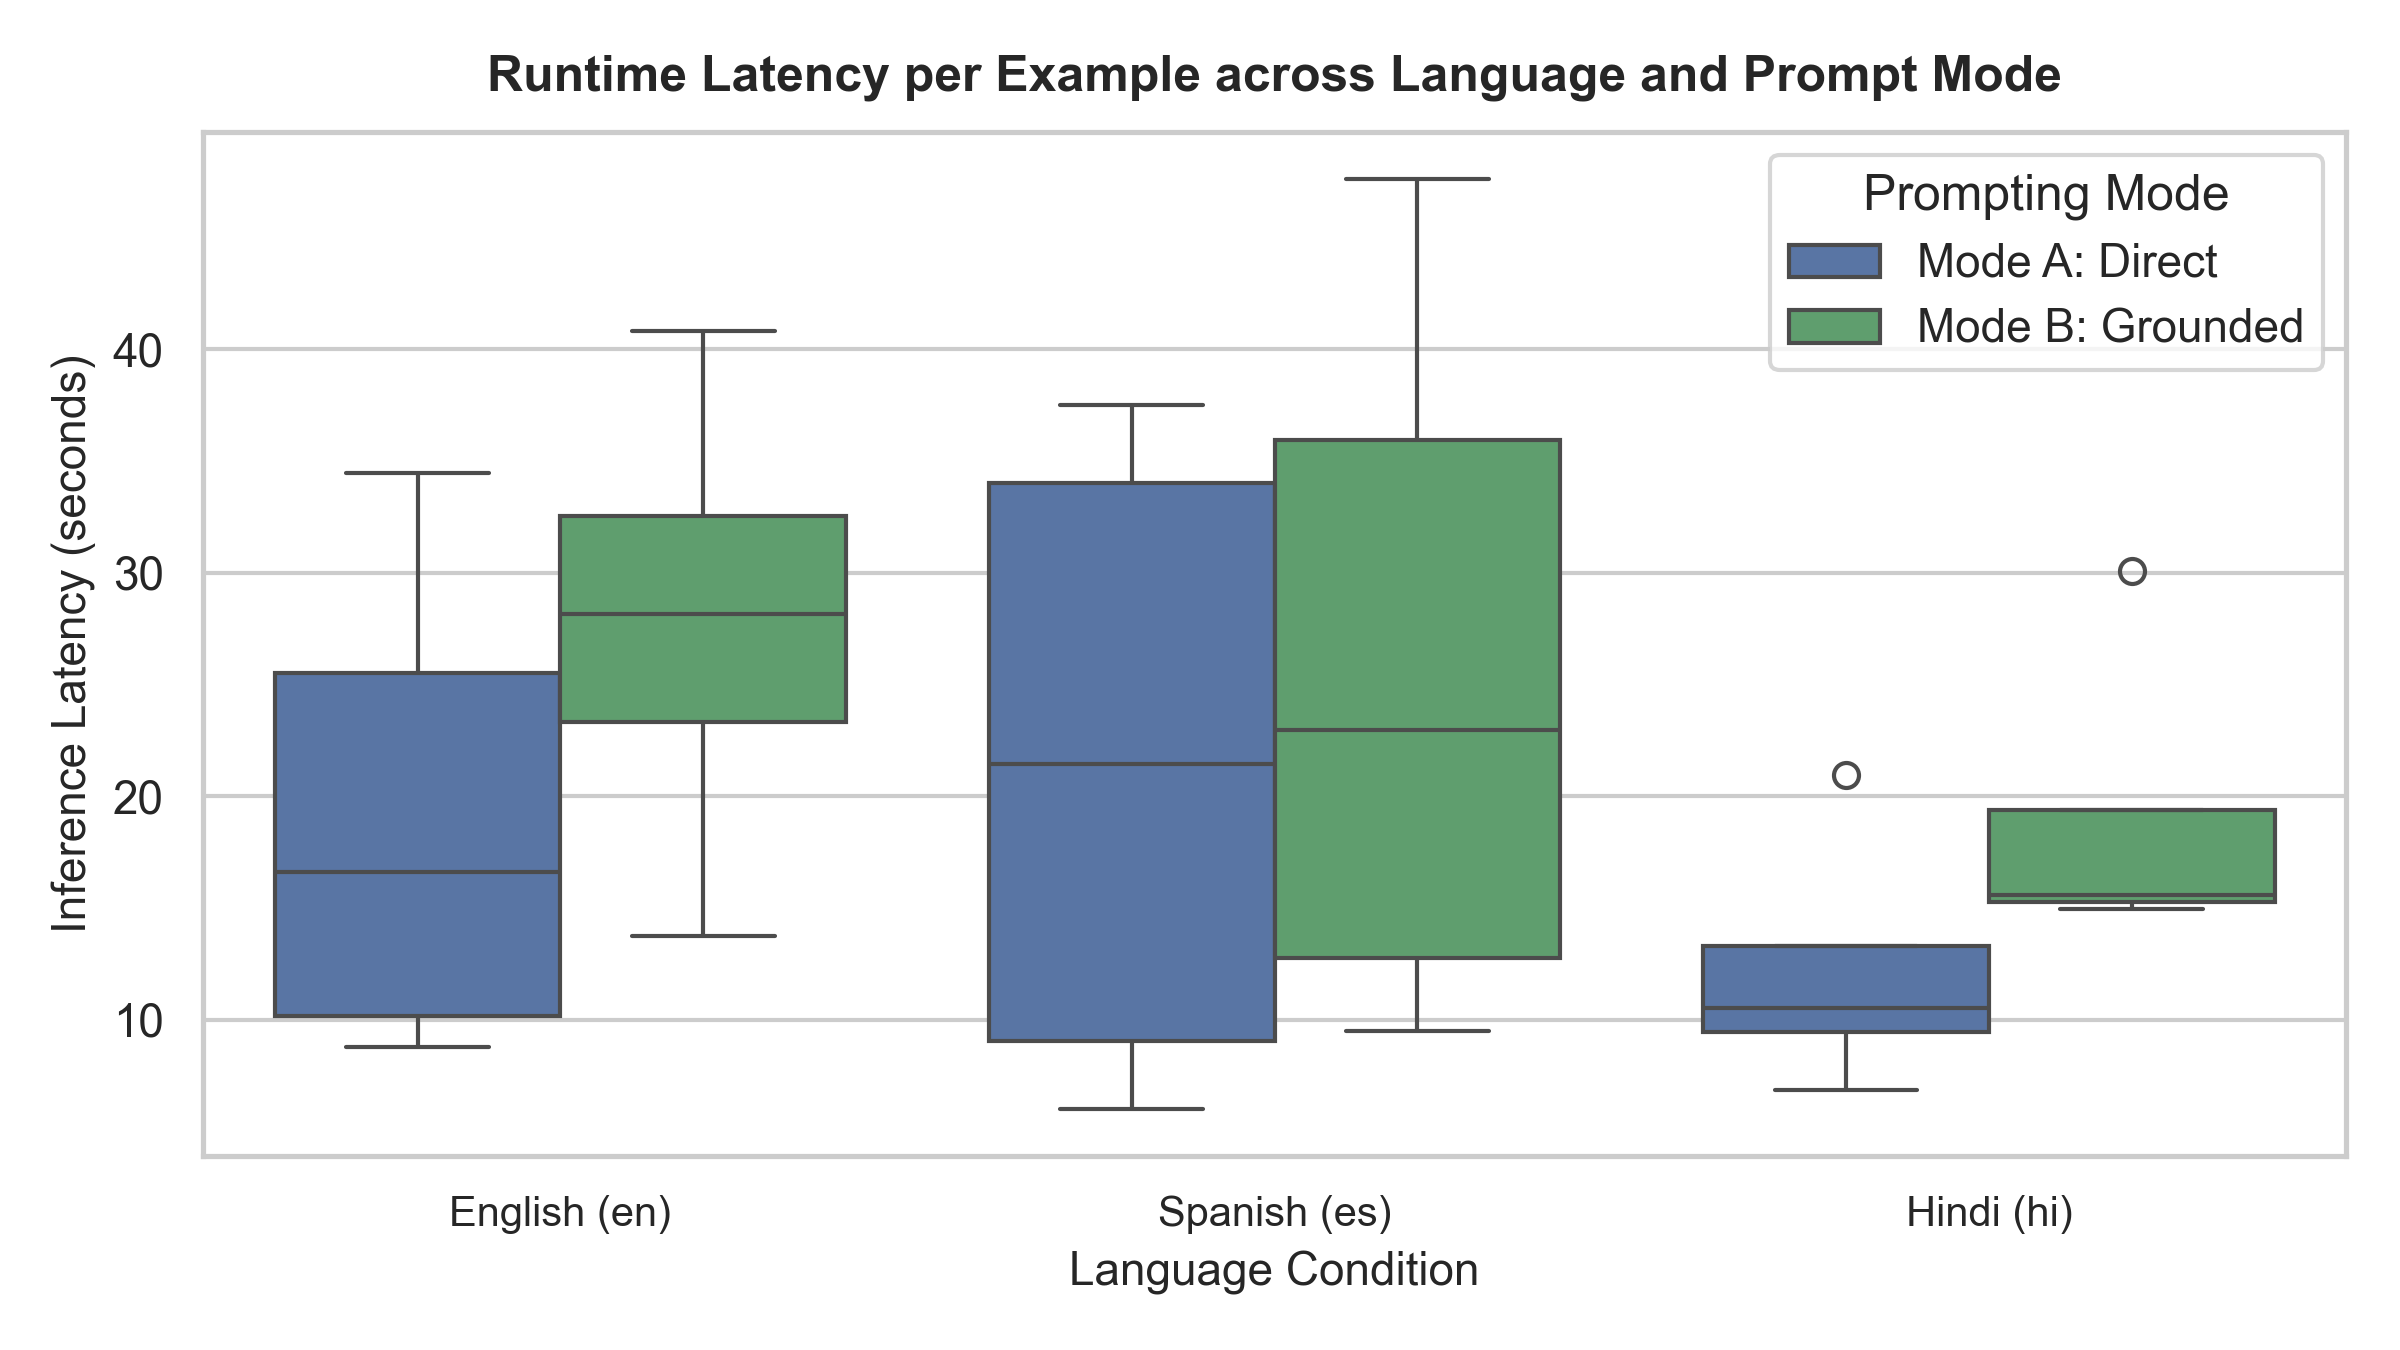
\includegraphics[width=\textwidth]{results/figures/fig3_runtime_by_condition.png}
        \caption{Inference latency distribution per example across conditions. Mode B requires $\approx 37\%$ more runtime than Mode A.}
        \label{fig:latency}
    \end{subfigure}
    \hfill
    \begin{subfigure}[b]{0.48\textwidth}
        \centering
        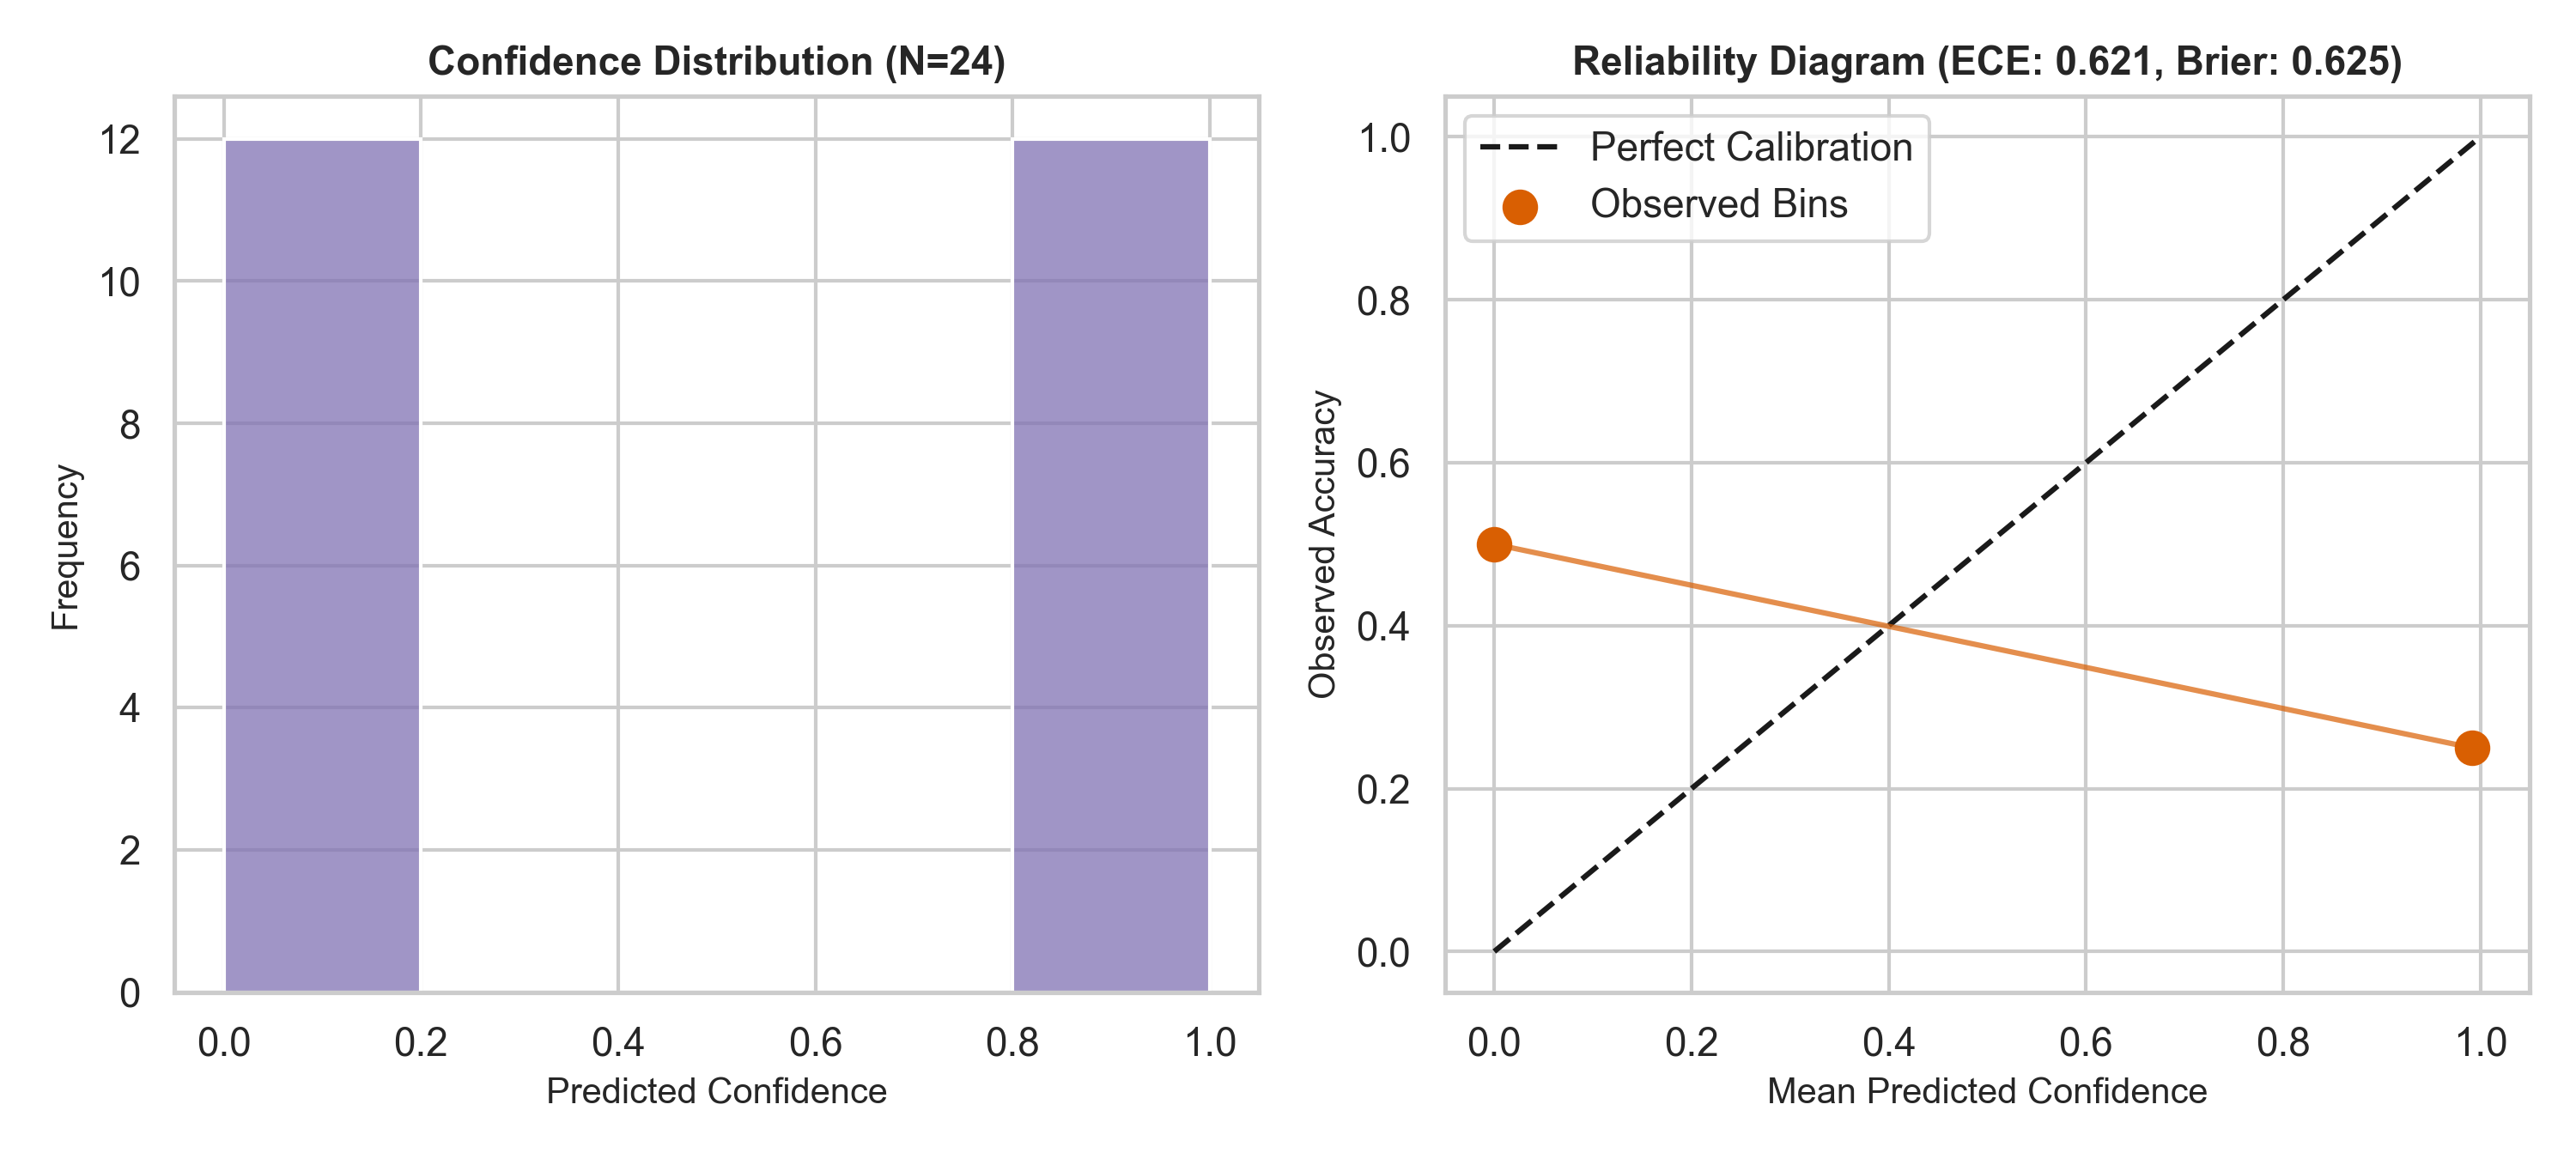
\includegraphics[width=\textwidth]{results/figures/fig5_calibration_analysis.png}
        \caption{Confidence histogram and reliability diagram. Verbalized confidence exhibits severe overconfidence ($\text{ECE} = 0.6208$).}
        \label{fig:calibration}
    \end{subfigure}
    \caption{Runtime efficiency and confidence calibration analysis.}
    \label{fig:runtime_and_calib}
\end{figure*}

\subsection{Confidence Calibration & Runtime Profiling}
Figure~\ref{fig:calibration} illustrates the empirical calibration of self-reported verbalized confidences. Across all 24 passes, the overall **Brier score was $0.6254$** and **Expected Calibration Error (ECE) was $0.6208$** ($\text{MCE} = 0.7417$). In Mode A, the model emitted a confidence of $1.00$ on all incorrect predictions, yielding an empirical calibration gap of $0.7417$. In Mode B, calibration improved to $\text{ECE} = 0.5000$.

Figure~\ref{fig:latency} profiles inference latency: Mode B required a mean latency of **$24.17\text{ s}$ per example**, representing a $37.0\%$ computational overhead compared to Mode A ($17.64\text{ s}$ per example), driven by longer generation lengths during rationale verbalization.

\section{Qualitative Error Analysis}
\label{sec:error_analysis}

To inspect the underlying failure mechanisms, we examine three qualitative case studies encompassing the full failure taxonomy.

\subsection{Case Study 1: Claim 1 (Doc 31715818) — Robust Abstention}
\begin{itemize}
    \item \textbf{Claim (EN):} ``0-dimensional biomaterials show inductive properties.''
    \item \textbf{Claim (HI):} ``0- विभिन्न जीव जीव- जीव-विज्ञानात्मक गुणों को दिखाता है'' (\textit{Transliteration:} ``0-vibhinn jeev-jeev-vigyanatmak gunon ko dikhata hai''; \textit{Literal gloss:} ``0- various bio-biological properties shows'').
    \item \textbf{Abstract (Doc 31715818):} Reviews nanotechnologies for stem cell tracking and scaffolds; zero mention of 0-dimensional inductive biomaterials.
    \item \textbf{Gold Annotation:} \texttt{NOT\_ENOUGH\_INFO}, Rationales: \texttt{[]}.
    \item \textbf{Model Output (All conditions):} \texttt{NOT\_ENOUGH\_INFO} (Correct).
    \item \textbf{Diagnosis:} The model successfully recognized the complete absence of inductive biomaterial evidence, abstaining across all three languages. Even when Hindi machine translation degraded into fragmented phrasing, the model did not hallucinate support.
\end{itemize}

\subsection{Case Study 2: Claim 3 (Doc 14717500) — Translation Drift & Multi-Hop Failure}
\begin{itemize}
    \item \textbf{Claim (EN):} ``1,000 genomes project enables mapping of genetic sequence variation consisting of rare variants with larger penetrance effects than common variants.''
    \item \textbf{Claim (HI):} ``1,000 भूविज्ञान परियोजना आनुवंशिक अनुक्रम परिवर्तनों का निर्माण करने में समर्थ करती है...'' (\textit{Transliteration:} ``1,000 bhu-vigyan pariyojana aanuvanshik anukram parivartanon ka nirmaan karne mein samarth karti hai...'').
    \item \textbf{Catastrophic Translation Drift:} MarianMT mistranslated ``genomes project'' into \textbf{``भूविज्ञान परियोजना''} (\textit{Transliteration:} ``bhu-vigyan pariyojana'', \textit{literally: Geology project})! In Hindi, \textit{bhu-vigyan} means Geology, whereas Genetics is \textit{jeenom}.
    \item \textbf{Abstract (Doc 14717500):} Discusses GWAS synthetic associations where rare variants account for common variant signals (sentences \texttt{[2]}, \texttt{[5]}, \texttt{[7]}).
    \item \textbf{Gold Annotation:} \texttt{SUPPORTS}, Rationales: \texttt{[2, 5]} and \texttt{[7]}.
    \item \textbf{Model Output (All conditions):} \texttt{NOT\_ENOUGH\_INFO} (Incorrect).
    \item \textbf{Diagnosis (\texttt{ERR_OTHER} / \texttt{ERR_TRANS_DRIFT}):} In English and Spanish, the model failed multi-hop deductive entailment over statistical genetics. In Hindi, translation drift fundamentally altered the domain from genomics to geology, making evidence grounding semantically impossible.
\end{itemize}

\subsection{Case Study 3: Claim 5 (Doc 13734012) — Mode Divergence & Rationale Omission}
\begin{itemize}
    \item \textbf{Claim (EN):} ``1/2000 in UK have abnormal PrP positivity.''
    \item \textbf{Abstract (Doc 13734012, Sent 4):} ``RESULTS Of the 32,441 appendix samples 16 were positive for abnormal PrP, indicating an overall prevalence of 493 per million population...''
    \item \textbf{Quantitative Equivalence:} $\frac{16}{32,441} \approx 4.93 \times 10^{-4} = 493 \text{ per million} \approx \frac{1}{2,028} \approx \frac{1}{2,000}$.
    \item \textbf{Gold Annotation:} \texttt{SUPPORTS}, Rationales: \texttt{[4]}.
    \item \textbf{Model Output Mode A:} \texttt{NOT\_ENOUGH\_INFO} (Failed).
    \item \textbf{Model Output Mode B:} \texttt{SUPPORTS} (Correct veracity across \texttt{en}, \texttt{es}, \texttt{hi}).
    \item \textbf{Diagnosis (\texttt{ERR_RAT_OMIT}):} Mode A collapsed to NEI. Mode B prompted sentence-level attention, allowing the model to perform the quantitative conversion ($493/\text{million} \approx 1/2000$). However, instead of outputting integer index array \texttt{[4]}, the model generated natural-language text (\textit{``The study aims to investigate...''}), resulting in $0.0\%$ Rationale F1.
\end{itemize}

\subsection{Failure Taxonomy Distribution}
Across the 24 pilot passes:
\begin{itemize}
    \item \textbf{\texttt{NONE} (Fully Correct):} $1/4$ instances in Mode A (Claim 1); $1/4$ instances in Mode B (Claim 1).
    \item \textbf{\texttt{ERR_RAT_OMIT} (Rationale Omission):} $1/4$ instances in Mode B across all languages (Claim 5).
    \item \textbf{\texttt{ERR_OTHER} (Conservative Over-Abstention):} $3/4$ instances in Mode A; $2/4$ instances in Mode B.
    \item \textbf{\texttt{ERR_POL_INVERT} (Polarity Inversion):} $0$ instances. The model never inverted \texttt{SUPPORTS} to \texttt{REFUTES}.
    \item \textbf{\texttt{ERR_NEI_FAIL} (False Certainty on NEI):} $0$ instances. The model never claimed false support when evidence was absent.
\end{itemize}

\section{Discussion}
\label{sec:discussion}

\subsection{The Mechanism of Abstention Collapse}
Our results uncover a fundamental limitation of direct zero-shot prompting (Mode A) in scientific fact verification: \textbf{conservative abstention collapse}. When confronted with an unsegmented scientific abstract, small models exhibit a strong prior toward \texttt{NOT\_ENOUGH\_INFO}, predicting abstention on $100\%$ of claims. Evidence-grounded prompting (Mode B) acts as a structural regularizer, decomposing the abstract into indexed sentences and forcing local attention over specific empirical findings.

\subsection{The Rationale Extraction Bottleneck}
While Mode B successfully unlocked positive veracity classification, it exposed a critical formatting bottleneck: zero-shot small language models fail to output clean integer index arrays. Instead, they verbalize explanations. Consequently, automated pipelines relying strictly on integer parsing will suffer severe rationale omission penalties (\texttt{ERR\_RAT\_OMIT}) unless guided by few-shot demonstrations or fine-tuned extraction heads.

\subsection{Translation Drift as a First-Order Threat in Indic NLP}
Our qualitative findings emphasize that machine translation remains a major failure mode for domain-specific scientific text. Translating ``1,000 genomes project'' into ``1,000 geology project'' demonstrates that generic NMT models trained on news or web corpora cannot be trusted for scientific literature analysis without domain adaptation or entity-constrained decoding.

\section{Limitations}
\label{sec:limitations}

We report the following limitations transparently:
\begin{enumerate}
    \item \textbf{Model Parameter Capacity:} We evaluated a compact 494M parameter causal LLM (\texttt{Qwen2.5-0.5B-Instruct}). Larger models (e.g., Llama-3-8B, Qwen-2.5-7B) possess richer representations and may exhibit different cross-lingual behaviors.
    \item \textbf{CPU Compute Constraint:} Local CPU inference latency averaged **$21.35\text{ seconds}$ per pass**. Evaluating the full 300-claim development set ($2,400$ passes) would require $\approx 14.2\text{ hours}$ of continuous CPU execution, necessitating a pilot-first protocol.
    \item \textbf{Statistical Power:} The pilot dataset evaluated 3 claims across 4 evaluation pairs ($N=24$ inferences). While sufficient to validate pipeline integrity, schema robustness, and identify catastrophic translation drift, inferential hypothesis tests (e.g., McNemar's test) remain directional rather than statistically definitive.
    \item \textbf{Unidirectional Evidence:} Evidence abstracts remained in English. A fully translated setup where abstracts are also translated would introduce additional compounding translation errors.
\end{enumerate}

\section{Conclusion}
\label{sec:conclusion}

This paper presented a controlled benchmark evaluating the multilingual factual reliability of large language models on scientific claim verification. By holding underlying biomedical evidence constant across English, Spanish, and Hindi, we demonstrated that evidence-grounded classification doubles veracity accuracy over ungrounded direct classification by breaking conservative abstention collapse. However, sentence-level rationale extraction remains a severe bottleneck, and machine translation introduces catastrophic terminological drift in lower-resource Indic scripts. Future work must focus on domain-adapted translation models and few-shot calibration to enable trustworthy multilingual scientific discovery.

\bibliographystyle{plain}
\bibliography{references}

\end{document}
